\documentclass[a4paper, 10pt, fleqn]{article}

\usepackage[utf8]{inputenc}
\usepackage[T1]{fontenc}
\usepackage{textcomp}
\usepackage{lmodern}
\usepackage[ngerman]{babel}
\usepackage{enumerate}
\usepackage{xcolor}

\usepackage{amsmath}
\usepackage{graphicx}
\usepackage{subcaption}
\usepackage{geometry}
\usepackage{scrpage2}
\usepackage{lastpage}
\usepackage[hyphens]{url}
\usepackage{hyperref}
\usepackage{listings}
\lstset{language=[ansi]C++}

\geometry{left=3cm, top=3cm, bottom=3cm, right=2cm}

\hypersetup{
    colorlinks,
    linkcolor={red!50!black},
    citecolor={blue!50!black},
    urlcolor={blue!80!black}
}


\pagestyle{scrheadings}
\ihead{PREN1 Gruppe 39}\ohead{Technologierecherche} 
\ifoot{\today} \ofoot{Seite \thepage\ von \pageref{LastPage}}


\begin{document}
% !TEX root = Konzeptvarianten.tex
\begin{titlepage}   

\begin{center}
\textsc{\Large PREN Team 39}\\[0.5cm]

% Title
\newcommand{\HRule}{\rule{\linewidth}{0.5mm}}
\HRule \\[0.4cm]
{ \huge \bfseries GüselStar XXI}\\[0.4cm]
{ \huge \bfseries Testat 2: }\\[0.4cm]
{ \LARGE \bfseries Evaluation der Lösungsprinzipien und Auswahl der optimalen Kombination(en)}\\[0.4cm]
\HRule \\[1.5cm]

% Author and supervisor
\begin{minipage}{0.4\textwidth}
\begin{flushleft} \large
\emph{Autoren:}\\
Patrizio Brantschen\\
Stefan Häfliger\\
Tobias Kreienbühl\\
Joël Meloni\\
Silvan Ritz\\
Lars Walther\\
Adrian Würsch
\end{flushleft}
\end{minipage}
\hfill
\begin{minipage}{0.4\textwidth}
\begin{flushright} \large
\emph{Team-Coach:} \\
Jürg Habegger
\end{flushright}
\end{minipage}

\vfill

% Unterer Teil der Seite
{\large \today}

\end{center}
\end{titlepage}
\tableofcontents
\clearpage
%% !TEX root = Technologierecherche.tex
\section*{Abstract}
%% !TEX root = Technologierecherche.tex
\section{Einleitung}
% !TEX root = Technologierecherche.tex
\section{Autonomes Fahren}
% !TEX root = Technologierecherche.tex
%\subsection{Spurerkennung}
%Damit das Fahrzeug die Strecke autonom abfahren kann, muss das Fahrzeug in der Lage sein, die Spur selbständig zu erkennen.
%Die autonome Spurerkennung kann mit unterschiedlichen mitteln realisiert werden.

\subsection{Erkennung des rechten Randes mit Sensoren}
Der rechte Rand des Parcours ist für die Spurerkennung vielversprechend. Er ist entweder durch eine weisse Linie, ein 5mm hohes Trottoir oder für kurze Zeit auf der Kreuzung nicht begrenzt.
Für die unterschiedlichen Bedingungen werden verschieden Möglichkeiten aufgezeigt.\\

\textbf {Erkennung der weissen Linie} \\
Die rechte Begrenzungslinie ist 1cm breit und weiss. Es gibt viele Minaturfahrzeuge die einer Linie folgen. Jedoch ist bei den meisten Linienfolger die zu folgende Linie in der Mitte des Fahrzeuges. Das hat der Vorteil das man links und rechts der Linie die Linie detektieren kann. Dies ist bei dieser Aufgabenstellung nicht oder nur sehr begrenzt möglich. Dies ist für beide Lösungsvarianten eine Herausforderung. Für beide wäre ein Funktionsmustr nötig.
Hier zwei Möglichkeiten:\\

\begin{figure} [hbp]
	\centering
	\begin{subfigure}[b]{0.4\textwidth}
		\includegraphics[width=\textwidth]{Images/Linienerkennung_1.png}
		\caption{Variante 1. Sensoren über der Linie}
	\end{subfigure}
	\hfill
	\begin{subfigure}[b]{0.42\textwidth}
		\includegraphics[width=\textwidth]{Images/Linienerkennung_2.png}
		\caption{Variante 2. Sensoren neben der Linie}
\end{subfigure}
	\caption{Mögliche Linienerkennungen mit Infrarotsensoren}\label{fig:animals}
\end{figure}

\textbf {Erkennung des Trottoirs}
Das Trottoir ist die längste und wichtigste (rechte) Begrenzung des Tracks. Es ist der längste Strassenabschnitt und die Positionsbestimmung muss a präzisesten funktionieren. Für das die Trottoir Erkennung sind diese zwei Varianten im Vergleich.\\
 
\begin{figure} [hbp]
	\centering
	\begin{subfigure}[b]{0.4\textwidth}
		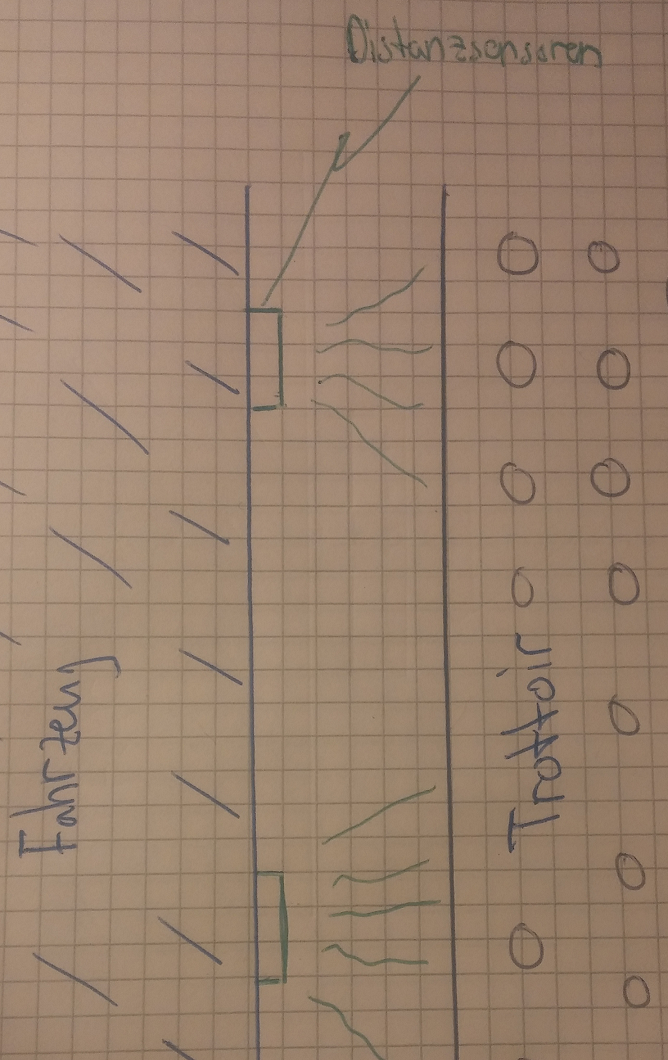
\includegraphics[width=\textwidth]{Images/Trottoirerkennung_1.png}
		\caption{Variante 1. Distanzsensoren als Abstandsmessung}
	\end{subfigure}
	\hfill
	\begin{subfigure}[b]{0.4\textwidth}
		\includegraphics[width=\textwidth]{Images/Trottoirerkennung_2.png}
		\caption{Variante 2. Distanzhalter als mechnische Bregrenzung (z.B Räder)}
\end{subfigure}
	\caption{Mögliche Spurhalte Konzepte beimTrottoir}\label{fig:animals}
\end{figure}

\textbf {Möglichkeiten bei keiner Begrenzung (Kreuzung)} \\
Die Kreuzung ist der Spezialfall des Tracks. Es gibt keine Begrenzung am rechten Rand. 
Da keine Begrenzung vorhanden ist, kann man mit Sensoren auch nicht detektieren.
Die Lösung ohne Sensoren ist bei der Kreuzung stur geradeaus zu fahren. Dies könnte man einprogrammieren, wenn weder eine Linie noch ein Trottior vorhanden ist. Dies setzt natürlich die richtige Ausrichtung des Fahrzeuges vor der Kreuzung voraus.\\

\subsection{Fest einprogrammierte Strecke ohne Sensoren}
Zu der Variante mit vielen Sensoren gibt es die Möglichkeit die Strecke fest einzuprogrammieren. Da die Strecke immer gleich bleibt (ausser den zwei Möglichen Startplätze) ist es Möglich die Strecke bereits fest einzuprogrammieren.
\textbf {Vorteile}
\begin{itemize}
\item Keine Sensoren für die Spurerkennung notwendig.
\item Kostenersparnis
\item Weniger Fehlerquellen\\
\end{itemize}
\textbf {Nachteile}
\begin{itemize}
\item Keine Fehlerkorrektur (einmal falsch, immer falsch)
\item Braucht extrem genauer Antrieb + Lenkung
\end{itemize}
% !TEX root = Technologierecherche.tex
\subsection{Rechtsvortritt}

% !TEX root = Technologierecherche.tex
\section{Beladen}
\subsection{1}
\subsection{2}
\subsection{3}
% !TEX root = Technologierecherche.tex
\section{Entladen}
\subsection{Kippen des Behälters}

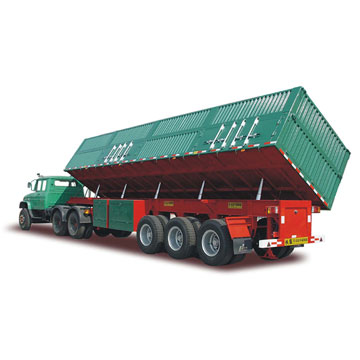
\includegraphics[width=0.5\textwidth]{Images/Entladen1.jpg}

Seitliches Entladen des Behälters

Vorteile:
\begin{itemize}
\item einfache Realisierung
\item wird in der Praxis angewandt
\end{itemize}

Nachteile:
\begin{itemize}
\item Nahes Heranfahren an Entladebehälter notwendig
\end{itemize}

\subsection{Seitliche Klappe öffnen}

Vorteil:
\begin{itemize}
\item sehr einfach realisierbar
\end{itemize}

\begin{flushleft}
Nachteile:
\end{flushleft}
\begin{itemize}
\item nicht automatisch wieder verschliessbar
\item fraglich ob Zielbereich einhaltbar ist
\end{itemize}

\subsection{Mit Greifer ausladen}

Vorteil:
\begin{itemize}
\item Greifer wird für 2 Funktion gebraucht (Einladen/Ausladen)
\end{itemize}

\begin{flushleft}
Nachteile:
\end{flushleft}
\begin{itemize}
\item schwierig gesamtes Schüttgut zu erwischen
\item aufwändiger Greifer
\item schwierig realisierbar
\end{itemize}
% !TEX root = Technologierecherche.tex
\section{Greifer}
\subsection{mechanisch}
Greifer besteht aus einer festen Seite und einer beweglichen Seite

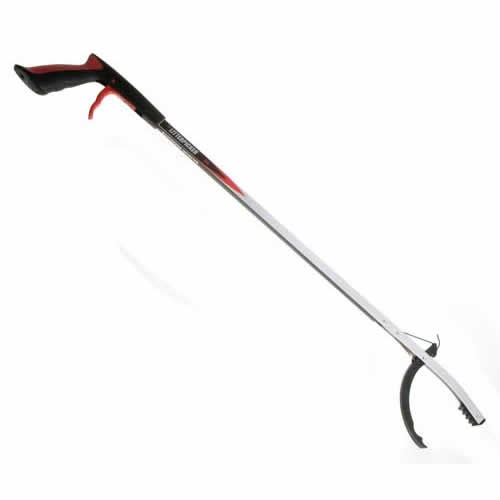
\includegraphics[width=0.5\textwidth]{Images/Gripper6.png}

Eigenschaften: 
\begin{itemize}
\item sehr einfacher Aufbau
\item wenige Teile notwendig
\item nicht präzise Lösung
\end{itemize}

Greifer mittels 2 Zahnräder gleichmässig schliessen

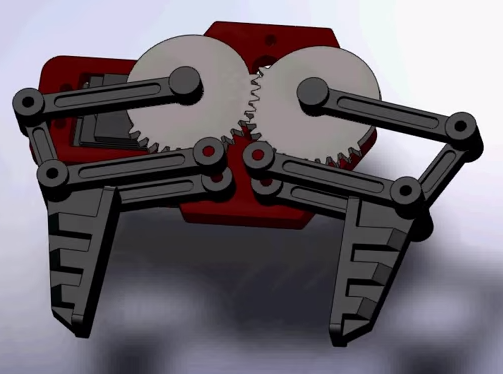
\includegraphics[width=0.5\textwidth]{Images/Gripper2.png}

Eigenschaften:
\begin{itemize}
\item präzise Lösung
\item aufwändiger Aufbau
\item symmetrischer Aufbau
\end{itemize}

\subsection{pneumatisch}
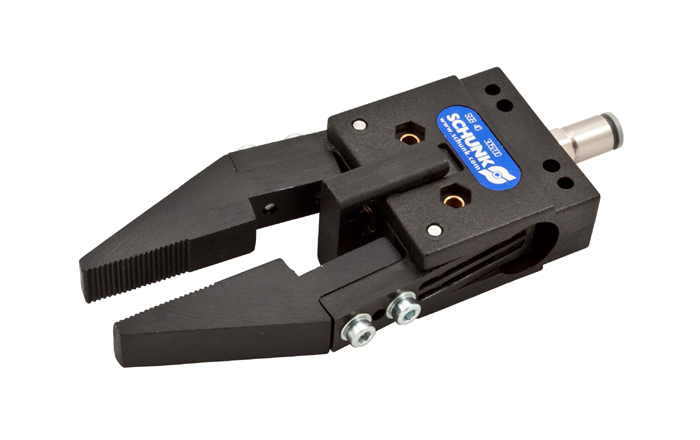
\includegraphics[width=0.5\textwidth]{Images/pneumatGr_schunk.jpg}

Eigenschaften: 
\begin{itemize}
\item Druckluft-Aggregat notwendig
\item hohe Präzision
\item teuer
\end{itemize}

\subsection{magnetisch}
Greifen der M4 Schrauben und Muttern mittels eines Elektromagneten

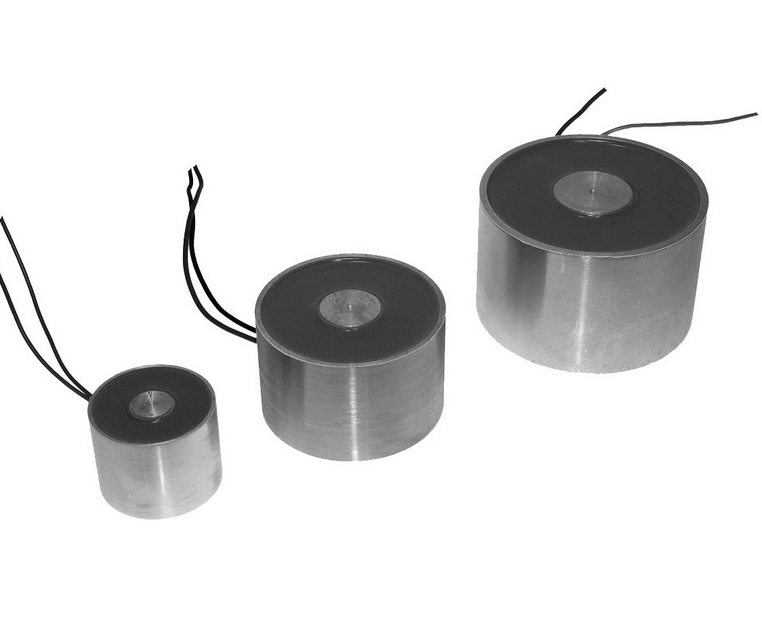
\includegraphics[width=0.5\textwidth]{Images/Magnetgreifer.png}

Eigenschaften:
\begin{itemize}
\item einfacher Aufbau
\item einfache Integration
\item fraglich ob genügend stark
\end{itemize}
% !TEX root = ../Dokumentation.tex
\subsection{Antrieb}

\textbf{Funktionsbeschrieb}\\[0.2cm]
Als Antrieb wird ein DC-Getriebemotor verwendet, der an der Unterseite montiert wird und für die Vor- sowie Rückwärtsbewegungen des Fahrzeugs zuständig ist.
Die aktuelle Drehzahl des Motors wird von einem Encoder erfasst. Dieser wiederum sendet die gemessenen Daten an den Microcontroller der schlussendlich die Anzahl Umdrehungen reguliert.\\[0.2cm]
\textbf{Komponentenbeschrieb}
\begin{figure}[H]
\centering
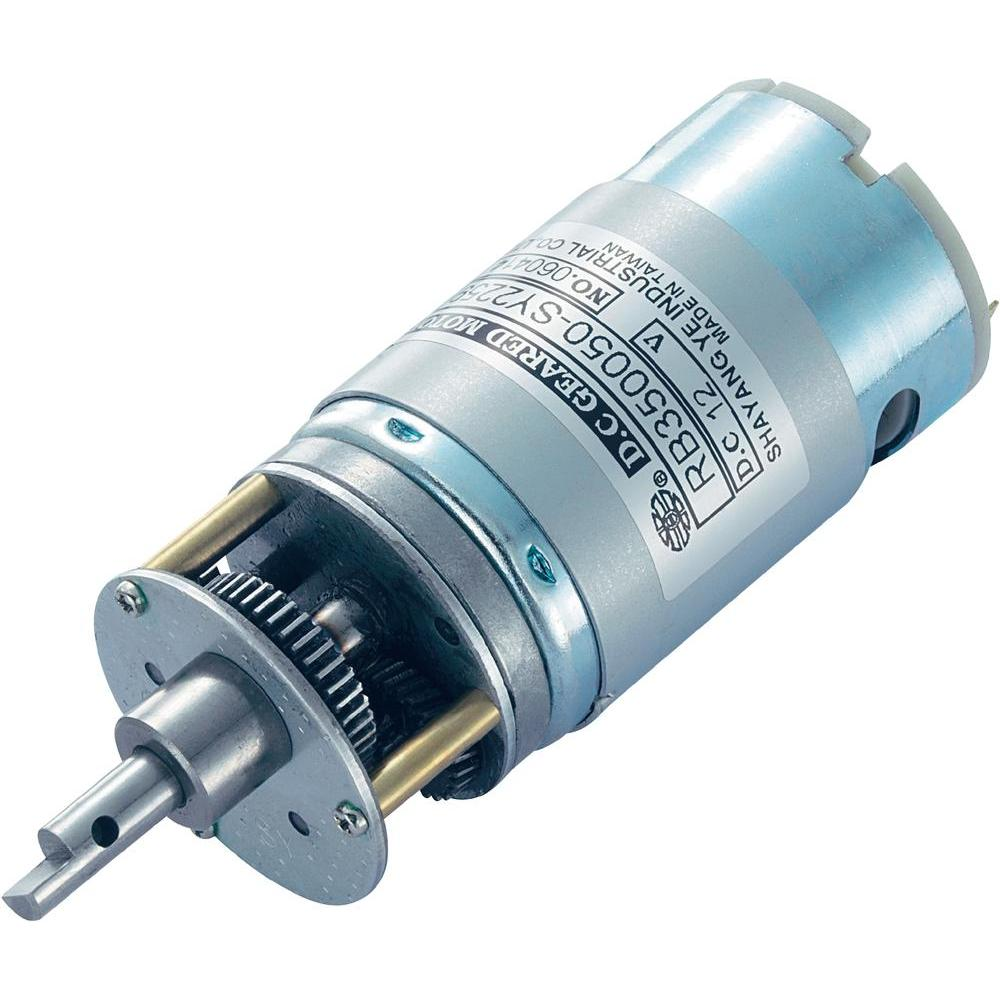
\includegraphics[width=0.5\textwidth]{03_Loesungskonzept/pictures/antrieb.jpg}
\caption{Antrieb  (Quelle:http://www.conrad.ch)}	
\end{figure}\flushleft
Als voraussichtlicher Favorit wurde ein Hochleistungsgetriebemotor von Modelcraft ausgewählt. Die technischen Daten sind folgende:
\begin{itemize}
\item Leerlaufstrom: 0.32 A
\item Last-Drehzahl: 317 U/min
\item Leerlauf-Drehzahl: 333 U/min
\item Betriebsspannung: 12 V DC
\item Spitzendrehmoment: 2.23 Nm
\item Max. Laststrom: 0.7 A
\end{itemize}
\textbf{Begründung}\\[0.2cm]
Der ausgewählte Motor punktet vor allem aufgrund seiner kleinen und kompakten Bauform. Da der Montageort für den Antrieb am Fahrzeug nicht verändert werden kann, ohne umständliche Wellen zu installieren, ist die Baugrösse relativ beschränkt.
Ein weiterer Punkt ist, dass er sich als Gleichstrommotor leicht ansteuern lässt und damit die Handhabung vereinfacht.
Zudem zeichnet er sich mit einer hohen Drehzahl und grossem Drehmoment aus und ist dennoch verhältnismässig günstig in der Anschaffung.

% !TEX root = Technologierecherche.tex
\section{Lenkung}
\subsection{Knicklenkung}
\begin{itemize}
\item Die Hinterachse volgt immer der gleichen Spur wie die Vorderachse.\\
\end{itemize}
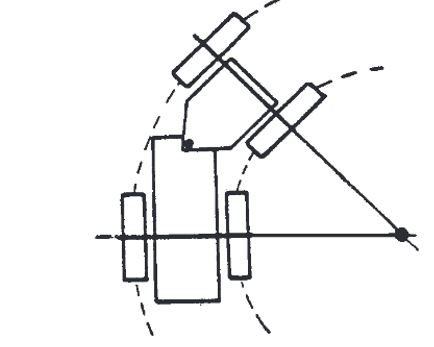
\includegraphics[width=0.5\textwidth]{Images/Knicklenkung.JPG}
\subsection{Achsschenkellenkung}
\begin{itemize}	
\item Die Standfestigkeit wird auch bei vollem Lenkeinschlag nicht beeinträchtigt.\\
\item Heutige zweiachsige PWS und Nutzfahrzeuge sind fast alle mit Achsschenkellenkung gebaut.\\
\item Das kurveninnere Rad ist stärker eingeschlagen als das kurvenäussere.\\
\end{itemize}
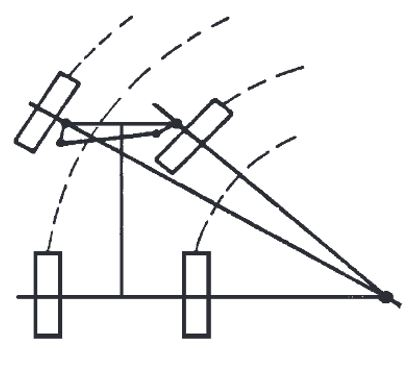
\includegraphics[width=0.5\textwidth]{Images/Achsschellenlenkung.JPG}
\subsubsection{Lenktrapez}
\begin{itemize}
\item Ermöglicht unterschiedliche Einschlagwinkel der Vorderräder.\\
\item Ermöglicht einfaches einstellen eines Spurwinkels.\\
\item Zur Berechnung von Lenktrapezen gibt es vorgefertigte EXEL Tabellen im Web.\\
\end{itemize}
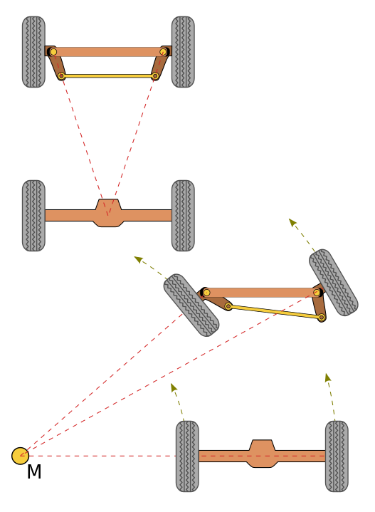
\includegraphics[width=0.5\textwidth]{Images/Lenktrapez.png}
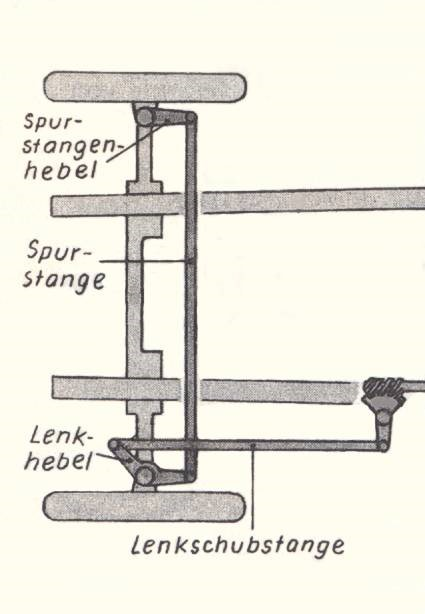
\includegraphics[width=0.5\textwidth]{Images/Lenktrapez2.jpg}
\subsection{Zweiradlenkung}
\begin{itemize}	
\item Lenkung mit einem Zwei- oder Dreiradfahrzeug durch unterschiedlich schnell rotierende Räder.\\
\end{itemize}
\subsection{Lenkung für Kettenfahrzeuge}
\begin{itemize}	
\item Die Lenkung kann durch unterschiedlich schnelles laufen lassen der Ketten realisiert werden.\\
\end{itemize}
% !TEX root = Dokumentation.tex
\section{Elektronische Bauteile}
\subsection {Motoren}
Hier kommt etwas über die Motoren rein.

\subsection*{MC Board}
\subsubsection{Anforderungen}
\begin{itemize}
\item Das Board muss eine Schnittstelle zu dem Boardcomputer haben.
\item Das Board muss AD Wandler haben.
\item Möglichst Kostengünstig.
\end{itemize}


\subsubsection{Tinkerforge}
%%Tinkerforge bietet ein vielseitiges System aus Mikrocontrollern, Sensoren, Treiber und weiteren Baugruppen an. Diese Funktionen sind jeweils in Module aufgeteilt, welche Modular hinzufügbar sind. Diese Module kommunizieren einerseits untereinander und andererseits mit einem Hauptsteuerelement. Dieses kann ein PC oder aber auch ein Linux basierter Minirechner sein (wie zum Beispiel das Beaglebone oder Freedomboard).\\\\%%
\textbf {Vorteile}
\begin{itemize}
\item Einfache und modulare Schnittstelle zum Boardcomputer.
\item Sehr einfach erweiterbar mit zusätzlichen Modulen (z.B Sensoren).\\
\end{itemize}
\textbf {Nachteile}
\begin{itemize}
\item Grosser Aufwand für eigene Module(Abhängigkeit zu Tinkerforge).
\item Eher teure Module.		
\end{itemize}
%%Mögliche Kostenberechnung: 1x Hauptmodul: 50, 2x Distanzsensoren: 10, Linesensor: 10, 2x Schrittmotoren: 100, Diverses:10. Gesamt: 180 Euro.%%

%%\begin{figure}[ht]
%%	\centering									
%%	\includegraphics{TinkerforgeUebersicht.jpg}
%%	\caption{Ein möglicher Aufbau des Tinkerfoge Systems. Hier mit einem Ultraschallsensor.}
%%	\label{fig1}
%%	%Quelle: http://www.heise.de/make/meldung/Modul-Baukasten-Tinkerforge-Abnabelung-vom-PC-dank-RED-Brick-2490601.html
%%\end{figure}

\subsubsection{HCS08 Devlopperboard}
%http://ch.farnell.com/freescale-semiconductor/dc9s08qe32/tochterplatine-f-r-demoqe32/dp/1692128

\subsubsection{MSP430 Launchpad}
%http://www.ti.com/ww/en/launchpad/launchpads-connected.html#tabs
\subsubsection{Arduinoboard}
%http://www.ti.com/ww/en/launchpad/launchpads-connected.html#tabs
\subsubsection{Freedomboard}
%http://www.ti.com/ww/en/launchpad/launchpads-connected.html#tabs

\subsection*{Distanzsensoren}
\subsubsection{Anforderungen}
\begin{itemize}
\item Einfaches auslesen der Daten muss möglich sein.
\item Genaue Positionsdaten, je nach Anforderungen +/- 1mm.
\item Preis darf 10Fr. nicht übersteigen.
\item Möglichst Störungsunabhängig.
\item Distanz 10cm.
\end{itemize}

\subsubsection{Ultraschallsensoren}
%Ultraschalsensoren werden häufig als Bewegungsmelder eingesetzt. 
%http://www.miniinthebox.com/de/ultraschall-modul-hc-sr04-entfernung-messumformer-sensor-fuer-arduino-201211270080054_p478889.html
\textbf {Vorteile}
\begin{itemize}
\item Erschwinglich, ein Sensor kostet ungefähr 5.Fr.
\item Häufig gebraucht für diese Anwendung => grosse Community.
\item Unempfindlich auf Störeinflüsse.(Ausser andere Ultraschallsensoren)
\item Kann als Liniensensor und Rad-Encoder eingesetzt werden.\\
\end{itemize}
\textbf {Nachteile}
\begin{itemize}
\item Kann als Liniensensor und Rad-Encoder eingesetzt werden.
\item Sind empfindlich auf UV-Licht!
\item Geringe Reichweite (je nach Typ nur bis 5mm)
\end{itemize}
\subsubsection{Infrarotsensoren}
%http://rn-wissen.de/wiki/index.php?title=CNY70
Infrarotsensoren eignen sich gut als Distanz oder Liniensensoren.\\
\textbf {Vorteile}
\begin{itemize}
\item Kostengünstig (Sensor und Empfänger kosten zusammen 1.7Fr).
\item Häufig gebraucht für diese Anwendung => grosse Community.
\item Kann als Liniensensor und Rad-Encoder eingesetzt werden.\\
\end{itemize}
\textbf {Nachteile}
\begin{itemize}
\item Benötigt zwei AD Eingänge.
\item Sind empfindlich auf UV-Licht!
\item Geringe Reichweite (je nach Typ nur bis 5mm)
\end{itemize}

\subsubsection{Liniensensoren/Reflexkoppler}
\end {document}

% !TEX root = Technologierecherche.tex
\section{Stromversorgung}

\subsection {Anforderungen}
\begin{itemize}
\item Muss die Energieversorgung gewährleisten können.
\item Darf sich aufgrund seiner Baugrösse und Gewichts nicht negativ auf das Fahrzeug auswirken
\end{itemize}

\subsection {Batterien}

\begin{itemize}
\item Einfache Beschaffung.
\item Günstig.
\item Relativ unempfindlich.
\item Platzsparende Montage möglich.
\item Einfache Energieregulierung durch Serie-, Parallelschaltung.
\item Geringe Selbstentladung.
\end{itemize}

\textbf {Nachteile}
\begin{itemize}
\item Nicht wieder aufladbar. 
\item Kurze Lebensdauer.	
\item Geringe Energiedichte.
\item Müssen regelmässig ersetzt werden.
\item Für den längeren und intensiven Gebrauch eher ungeeignet
\end{itemize}

\subsection {NiCd (Nickel-Cadmium)}

\begin{itemize}
\item Grosse Auswahl an verschiedenen Bauformen.
\item Billig.
\item Lange Lebensdauer.
\item Relativ unempfindlich.
\item Simple und billige Ladegeräte.
\end{itemize}

\textbf {Nachteile}
\begin{itemize}
\item Relativ schwer.
\item Geringe Energiedichte.
\item Mittelmässiger Ladewirkungsgrad.
\end{itemize}

\subsection {Lithium-Akku (LiPo, Lilon)}

\begin{itemize}
\item Grosse Auswahl von verschiedenen Bauformen.
\item Sehr hohe Energiedichte.
\item Geringe Selbstentladung.
\item Lange Lebensdauer.
\item Hoher Ladewirkungsgrad.
\item Relativ leicht.
\end{itemize}

\textbf {Nachteile}
\begin{itemize}
\item Empfindlich bei Über- und Unterschreiten der Spannungsgrenze.
\item Teuer.	
\item Benötigt teure Ladegeräte.	
\end{itemize}

\subsection {NiMH (Nickel-Metallhydrid)}
\begin{itemize}
\item Billig.
\item Lange Lebensdauer.
\item Relativ unempfindlich.
\item Simple und billige Ladegeräte.
\end{itemize}

\textbf {Nachteile}
\begin{itemize}
\item Relativ schwer.
\item Mittelmässige Energiedichte.
\item Mittelmässiger Ladewirkungsgrad.
\end{itemize}


% !TEX root = Konzeptvarianten.tex
\section{Boardcomputer}

Bei den Boardcomputern beschränkte sich die Recherche auf die Raspberry-Familie.
Diesem Mini-Computer geht ein gewisser Ruf voraus, der gewiss nicht unbegründet ist.
Ausserdem wurde er bisher in fast jedem PREN verwendet, da er für sehr viele Anwendungsbereiche eingesetzt werden kann.
Zusätzlich kennen sich einzelne Teammitglieder bereits ein wenig damit aus.
In die engere Auswahl kamen das Raspberry Pi (Pi), das Raspberry Pi 2 (Pi2) und das Banana Pi (BPi).


\begin{table}[h]
\begin{tabular}{|p{4.5cm}|p{3.5cm}|p{2cm}|p{2cm}|p{2cm}|}\hline
	
	\textbf{Kriterium}	& 	\textbf{Gewichtung (1-3)} & \textbf{Pi} & \textbf{Pi 2} & \textbf{BPi}\\\hline
	{Preis}	& 	{2} & {2} & {3} & {1}\\\hline
	{Grösse}	& 	{2} & {2} & {2} & {1}\\\hline
	{Leistung}	& 	{3} & {2} & {3} & {1}\\\hline
	{Ansteuerung}	& 	{2} & {3} & {3} & {2}\\\hline
	
	
	
	
\end{tabular}\\
\end{table}
% !TEX root = Dokumentation.tex
\section{Bilderkennung}

\subsection {Anforderungen}
\begin{itemize}
\item Objekterkennung (Container, Fahrzeug von rechts).
\item Linie erkennen.
\item Winkel der Linie erkennen.
\item Farbe erkennen.
\item Muss auf Linux oder Windows lauffähig sein.
\item Muss mit Java, C++ oder C-Sharp kompatibel sein.
\item Muss gut dokumentiert sein oder eine gute Community haben.
\end{itemize}

\subsection {OpenCV}

\begin{itemize}
\item Läuft auf den meisten Plattformen.
\item Stellt eine grosse Bibliotheke mit vielen Zusatzmodulen zur Verfügung.
\item Ist mit vielen grossen anderen Bibliotheken kompatibel.
\item Hat eine grosse Community.
\item Ist gratis und open source (BSD) lizenziert.
\item Ist gut dokumentiert.
\item Ist kompatibel mit Java, C, C++, Python usw..
\item Läuft sehr schnell.
\end{itemize}

\textbf {Nachteile}
\begin{itemize}
\item Enthält auch viele Funktionalitäten, welche nicht benötigt werden (komplex).		
\end{itemize}

\subsection {SimpleCV}

\begin{itemize}
\item Läuft auf den meisten Plattformen.
\item Ist mit OpenCV kompatibel.
\item Ist gratis und open source.
\item Hat eine grosse Community.
\item Ist gut dokumentiert.
\item Ist kompatibel mit Python.
\item Läuft schnell.
\item Leicht zu erlernen.
\end{itemize}
\textbf {Nachteile}
\begin{itemize}
\item Deckt möglicherweise nicht alle Anforderungen.	
\end{itemize}

\subsection {LibCCV}
\begin{itemize}
\item Läuft auf allen Plattformen.
\item Ist gratis und open source (BSD) lizenziert.
\end{itemize}
\textbf {Nachteile}
\begin{itemize}
\item Die Dokumentation ist mässig.
\end{itemize}





% !TEX root = Technologierecherche.tex
\section{Kamerasysteme}
\subsection{Raspberry Pi CAM}
\begin{itemize}
\item Kosten: $\pm$30.-
\item Baugrösse: 25x20x9mm
\item Auflösung: 5 Megapixel, bis 30 Bilder pro Sekunde, 1080x720 HD
\item Schnittstelle: 15 Pin Flachband MIPI Kameraschnittstelle.
\item Lieferzeit: Innert 24h (Digitec)
\item Kamerawinkel Horizontal: 53.5 $\pm$ 0.13 Grad.
\item Kamerawinkel Vertikal: 41.41 $\pm$ 0.11 Grad.
\item Bildformate: JPEG (beschleunigt), JPEG + RAW, GIF, BMP, PNG, YUV420, RGB888
\item Brennweite: 3.6mm $\pm$ 0.01
\item Fixer Fokus: 1m bis unendlich
\item Software: keine, Kompatibel zu RaspberryPi 1 und 2
\end{itemize}
\subsection{Logitech Webcam C525}
\begin{itemize}
\item Kosten: $\pm$70.-
\item Baugrösse: 60x 40x 20mm geschätzt, keine genauen Angaben auf Herstellerseite.
\item Auflösung: 8 Megapixel, 1280x720 HD
\item Schnittstelle: USB 2.0
\item Lieferzeit: Innert 24h (Fust, Microspot, Logitech)
\item Kamerawinkel Horizontal: Keine Angaben
\item Kamerawinkel Vertikal: Keine Angaben
\item Bildformate: Keine Angaben
\item Brennweite: Keine Angaben
\item Fokus: Autofokus
\item Software: Logitech Software nur Windows Vista, 7 und 8.
\end{itemize}
\subsection{Logitech Webcam C615}
\begin{itemize}
\item Kosten: $\pm$100.-
\item Baugrösse: 80x 40x 20mm geschätzt, keine genauen Angaben auf Herstellerseite.
\item Auflösung: 8 Megapixel, 1920x1080 Full HD
\item Schnittstelle: USB 2.0
\item Lieferzeit: Innert 24h (Fust, Microspot, Logitech)
\item Kamerawinkel Horizontal: Keine Angaben
\item Kamerawinkel Vertikal: Keine Angaben
\item Bildformate: Keine Angaben
\item Brennweite: Keine Angaben
\item Fokus: Autofokus
\item Software: Logitech Software nur Windows Vista, 7 und 8.
\end{itemize}
\subsection{Logitech Webcam C920}
\begin{itemize}
\item Kosten: $\pm$100.-
\item Baugrösse: 80x 40x 20mm geschätzt, keine genauen Angaben auf Herstellerseite.
\item Auflösung: 5 Megapixel, 1080x720 HD
\item Schnittstelle: USB 2.0, VID\_046D{\&}PID\_0821
\item Lieferzeit: Innert 24h (Fust, Microspot, Logitech)
\item Kamerawinkel Diagonal: 83 Grad
\item Kamerawinkel Vertikal: Keine Angaben
\item Bildformate: Keine Angaben
\item Brennweite: 4.3mm
\item Fokus: Autofokus
\item Software: Logitech Software nur Windows Vista, 7, 8 und 10.
\end{itemize}
\subsection{Logitech QuickCAM Series}
% !TEX root = Technologierecherche.tex

\subsection{Steuerung}
Die Steuereinheit ist Haupteinheit für das autonome Fahren. In der Steuerung werden die Spurdaten eingelesen, verarbeitet und die entsprechenden Massnahmen getroffen. Ohne eine gute Steuerung ist das autonome Fahren nicht möglich. 
\subsection{Ein Steuerungsboard}
Ein Board für die Verarbeitung der Spurdaten und für den Zugriff auf die Peripherie.
\textbf {Vorteile}
\begin{itemize}
\item Keine Kommunikationsschnittstelle nötig (Fehlerquelle eliminiert)
\item Preisersparnis\\
\end{itemize}
\textbf {Nachteile}
\begin{itemize}
\item Arbeitsaufteilung schwierig
\item Weniger Rechenperformance
\end{itemize}

\subsection{Bordcomputer und Hardwarecontroller}
Ein Board für die Verarbeitung der Spurdaten und Steuerung und ein anderes Board für den Zugriff auf die Peripherie und alternative Aufgaben.
\textbf {Vorteile}
\begin{itemize}
\item Getrennte Aufgabenbereiche 
\item Genügend Rechenperformance
\item Weniger Seiteneffekte\\
\end{itemize}
\textbf {Nachteile}
\begin{itemize}
\item Braucht zwei Boards
\item Schnittstelle nötig
\end{itemize}
% !TEX root = Technologierecherche.tex
\section{Morphologischer Kasten}
\begin{table}
\begin{tabular}{|l|l|l|l|l|}
\hline
Energieversorgung & Elektrisch (Akku) & Brennstoff & Pneumatik (direkt) & Pneumatik (Drucktank)\\\hline
Startsignal & Knopf & Laptop & Smartphone\\\hline
Stoppsignal & Akustisch & Licht (Blinken) & Laptop Rück & Smartphone Rück\\\hline
Antrieb & Elektromotor & Verbrennungsmotor & Pneumatik (Drucktank)\\\hline
Lenkung & Trapezlenkung & Achsenlenkung & Raupenlenkung & MC Car\\\hline
Chassis & 2 Achsen 4 Räder & 2 Raupen & 2 Räder 1 Stütze\\\hline
Anhalten & Bremsen & Motor stoppen\\\hline
Spurerkennung & Optisch & Infrarot & Ultraschall\\\hline
Containererkennung & Optisch & Infrarot & Ultraschall & Farbsensor (z.B. Lego)\\\hline
Greifen & Gelenkarm & Kettengreifer\\\hline
Leerung & Schräge & Kippen & Stossen\\\hline
Lagerung & Becken & Beweglicher Container	\\\hline
\end{tabular}\\
\caption{Morphologischer Kasten}
\end{table}
% !TEX root = Technologierecherche.tex
\section{Recherchequellen}



\begin{table}[h]
\begin{tabular}{|p{3cm}|p{3.5cm}|p{5cm}|p{2cm}|}\hline
	
	\textbf{Themengebiet}	& 	\textbf{Beschreibung} & \textbf{Quelle} & \textbf{Bewertung (1-5)} \\\hline
	
	
	\textbf{Bilderkennung}	&	OpenCV Beschreibung	&	\url{http://docs.opencv.org/master/d1/dfb/intro.html#gsc.tab=0}	&	3 \\\hline
				 			&	Vergleich von OpenCV und SimpleCV	&	\url{http://simplecv.tumblr.com/post/19307835766/opencv-vs-matlab-vs-simplecv}	&	4 \\\hline
				 			&	SimpleCV Beschreibung	&	\url{http://simplecv.org/}	&	3 \\\hline
				 			&	Linienerkennung mit Open CV	&	\url{https://www.youtube.com/watch?v=aGGehlgiZoQ}	&	3	\\\hline
				 			
\textbf{Boardcomputer}	& 	Raspberry Pi & \url{https://www.pi-shop.ch/raspberry-pi-model-b} & 4 \\\hline
						& 	Raspberry Pi 2 & \url{https://www.pi-shop.ch/raspberry-pi-2-model-b} & 4 \\\hline
						& 	Banana Pi & \url{https://www.pi-shop.ch/banana-pi} & 4 \\\hline	
						
\textbf{Antrieb}	& 	Elektromotor & \url{http://www.modellbau-friedel.com} & 3 \\\hline
					& 	Verbrennungsmotor & \url{http://www.modellbau-friedel.com} & 3 \\\hline
					& 	Dampfmaschine & \url{www.modell-dampfmaschinen.de} & 3 \\\hline
					
\textbf{Lenkung} &  Beschreibung Knicklenkung und Bild & \url{http://www.portmanns.ch/Repetition/Fahrwerk/Lenkungsarten.pdf} & 3 \\\hline

& Beschreibung und Bild Achsschenkellenkung & \url{http://www.urlaub-und-hobby.de/metallbaukasten/so09dt.html} & 4 \\\hline 

& Lenktrapez & \url{http://portmanns.ch/Repetition/Fahrwerk/Achssch.pdf} & 2 \\\hline 

\textbf{Stromversorgung}	&	Vergleich von Akkutypen	&	\url{http://www.akku-abc.de/akku-vergleich.php}	&	3 \\\hline
				 			&	Grundlagenbeschreibung Akkutypen 	&	\url{http://rn-wissen.de/wiki/index.php/Akku-Grundlagen}	&	4 \\\hline
				 			&	Vergleich von Batterien und Akkus	&	\url{http://www.conrad.de/ce/de/content/ti_AkkusBatterien/Nickel-Zink-Akkus-die-neue-Alternative-zu-den-herkoemmlichen-Batterien}	&	3 \\\hline
				 			&	Vergleich von Batterien und Akkus	&	\url{http://www.computerbild.de/artikel/cb-Tests-PC-Hardware-Teure-Marken-gegen-Billig-Batterien-Mignon-AA-Micro-AAA-4640760.html } & 2	\\\hline
 
	
\end{tabular}\\
\caption{Recherchequellen}
\end{table}
%% !TEX root = Technologierecherche.tex
\section{Schluss}
\end{document}